% control regions, transfer factors
% binning in razor variables
% statistical treatment and systematic uncertainties


In light of the discussion in Section~\ref{sec:boost_motivation}, it is expected that boosted top
quarks are a promising signature of new physics involving a massive gluino decaying to a relatively
light top squark.
Boosted objects with high transverse momentum are characterized by merged decay products
separated by $ \Delta R {\sim} 2 m / \pt $\footnote{Considering a heavy object $\W$ with mass $M$
that decays to two massless particles $a$ and $b$, we find $M^2 = 2 p_a \cdot p_b = 2 E_a E_b (1
- \cos{\theta_{ab}})$. Using small angle approximation this becomes $M^2 = E_a E_b
\theta_{ab}^2$. Assigning half of the $\W$ energy to both $a$ and $b$ results in $M^2 =
\frac{1}{4} E_\W^2 \theta_{ab}^2$. Translating this relation into the transverse plane, we get
$\Delta R = \frac{2 M}{\pt^\W}$.}, 
where $m$ and $\pt$ denote the mass and transverse momentum of the mother particle, and $\Delta R$
is given in terms of azimuthal angle $\phi$ and pseudorapidity $\eta$ as $\Delta R = \sqrt{\Delta
\phi^2 + \Delta \eta^2}$.
For a separation of $\Delta R = 0.5$, a top quark should thus have a momentum of ${\sim}700$\GeV, a
value difficult to reach with proton-proton collisions at 8 TeV. Therefore, in order to increase the
signal efficiency, we consider instead $\W$ bosons from top quark decays, which are required to have
a more accessible $\pt {\sim} 320$\GeV.  The final state we target will therefore contain boosted
$\W$ bosons and jets originating from $\cPqb$ quarks (i.e. $\cPqb$ jets).
Hadronically decaying boosted $\W$ boson candidates will be identified using pruned jet
mass~\cite{Ellis:2009su,Ellis:2009me,Chatrchyan:2013vbb} and a jet substructure observable
called N-subjettiness \cite{Thaler:2010tr}. More details on the \W tagging technique will be given
in Section~\ref{sec:boost_wtag}. 

The razor kinematic variables \mr and \rsq, see Section~\ref{sec:boost_razor}, are designed to
discriminate processes with new heavy particles and missing energy from standard model processes.
They will be used in this analysis as the main discriminating variables to search for deviations
from the SM. We will perform the search in 25 search bins across the high $\mr$-high $\rsq$ region,
using hadronic events with at least one boosted $\W$ boson and one $\cPqb$ jet.  

Standard model backgrounds in the signal regions are estimated using observations in control regions
and global scale factors, calculated from simulated data, that relate the number of events in one
region to that in another. 
Three control regions, $Q$, $W$, and $T$, are defined to select high-purity samples of multijet,
$\W(\rightarrow \ell\nu)+$jets and $t\bar{t}$ processes, respectively.  
The background estimation method uses a likelihood-based approach, and a simultaneous sampling
of systematic uncertainties which fully takes into account any correlations automatically.
An overview of the different regions and how they are related, including for the control regions
which background parameters of the likelihood each region constrains, is shown in
Fig.~\ref{fig:boost_flowchart}. For the full explanation of the background estimation method, I
refer to Section~\ref{sec:boost_likelihood}. 

\begin{figure}[p]
  \centering
  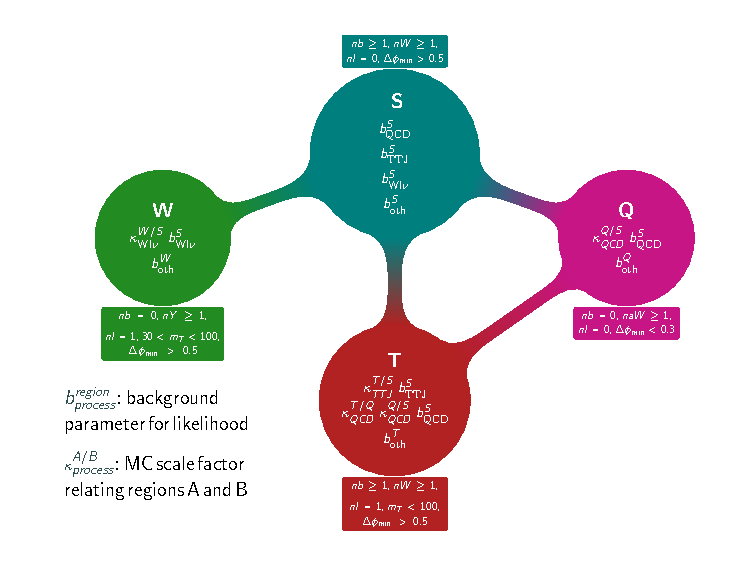
\includegraphics[width=\textwidth]{figures/razor_strategy/BoostFlowChart_noZ}
  \caption{Definition of, and relationship between, the signal ($S$) and control ($Q,T,W$) regions
and their relationship to the bin-by-bin background parameters
$b^{\textrm{region}}_{\textrm{process}}$ for a given region and background process, as well as the
four global scale factors $\kappa^{A/B}_{\textrm{process}} = \sum_i b^A_{\textrm{process}, MC, i} /
\sum_i b^B_{\textrm{process}, MC, i}$, where the sum is over all 25 (\mr,\rsq) bins of the simulated
data. 
The total expected background, per bin, is the sum of the terms shown for each region. Furthermore,
associated with each bin of each region is an observed count $N^{\textrm{region}}$, a simulated
count $N^{\textrm{region}}_{\textrm{process}, MC}$, and a count $N^{\textrm{region}}_{oth, MC}$
equal to the sum of the smaller backgrounds, with associated parameter $b^{\textrm{region}}_{oth}$.
  \label{fig:boost_flowchart}}
\end{figure}
